%------------------------------------------------------------------------------
%
% LaTeX-mall för examensarbeten vid LNU
% Skapad av Marcus Wilhelmsson, Institutionen för Datavetenskap
% Fakulteten för Teknik
% Linnéuniversitetet
%
% Licens: Creative Commons BY
%
% 
%------------------------------------------------------------------------------
%
%------------------------------------------------------------------------------
%	Inställningar och dokumentkonfiguration
%------------------------------------------------------------------------------

\documentclass[a4paper,12pt]{article} % A4-sida och 12 punkters fontstorlek


\usepackage[T1]{fontenc} % 8-bitarskodning som har 256 glyfer
\usepackage{times} % Typsnitt i dokumentet
\usepackage[swedish,english]{babel} % Svenskt språk, engelska för extra abstract
\usepackage[utf8]{inputenc} % För svenska tecken (UTF-8)
\usepackage{dtklogos} % Logos för t.ex. LaTeX, BibTeX, etc.
\usepackage{wallpaper} % Bakgrundsbild
\usepackage[absolute]{textpos} % Möjlighet att absolutpositionera text
\usepackage[top=2cm, bottom=2.5cm, left=3cm, right=3cm]{geometry} % Ställ in marginaler
\usepackage{appendix} % Stöd för separat hantering av bilagor
\usepackage{cite}
\usepackage{listings}
\usepackage[hidelinks]{hyperref}
\usepackage{float}


\setcounter{secnumdepth}{3} % Fem nivåer av underrubriksnumrering
\setcounter{tocdepth}{3} % Fem nivåer av underrubriksnumrering i innehållsförteckning

\usepackage{sectsty} % Ändra storlek på section och subsection till 12 punkter
\sectionfont{\fontsize{14}{15}\selectfont}
\subsectionfont{\fontsize{12}{15}\selectfont}
\subsubsectionfont{\fontsize{12}{15}\selectfont}

\usepackage{csquotes} % Används för att hantera citat


%------------------------------------------------------------------------------
%	Denna del används för att skapa boxen med författare, handledare, etc.

\newsavebox{\mybox}
\newlength{\mydepth}
\newlength{\myheight}

\newenvironment{sidebar}%
{\begin{lrbox}{\mybox}\begin{minipage}{\textwidth}}%
{\end{minipage}\end{lrbox}%
 \settodepth{\mydepth}{\usebox{\mybox}}%
 \settoheight{\myheight}{\usebox{\mybox}}%
 \addtolength{\myheight}{\mydepth}%
 \noindent\makebox[0pt]{\hspace{-20pt}\rule[-\mydepth]{1pt}{\myheight}}%
 \usebox{\mybox}}

%------------------------------------------------------------------------------
%	Titel-sektion
%------------------------------------------------------------------------------
\newcommand\BackgroundPic{
    \put(-2,-3){
    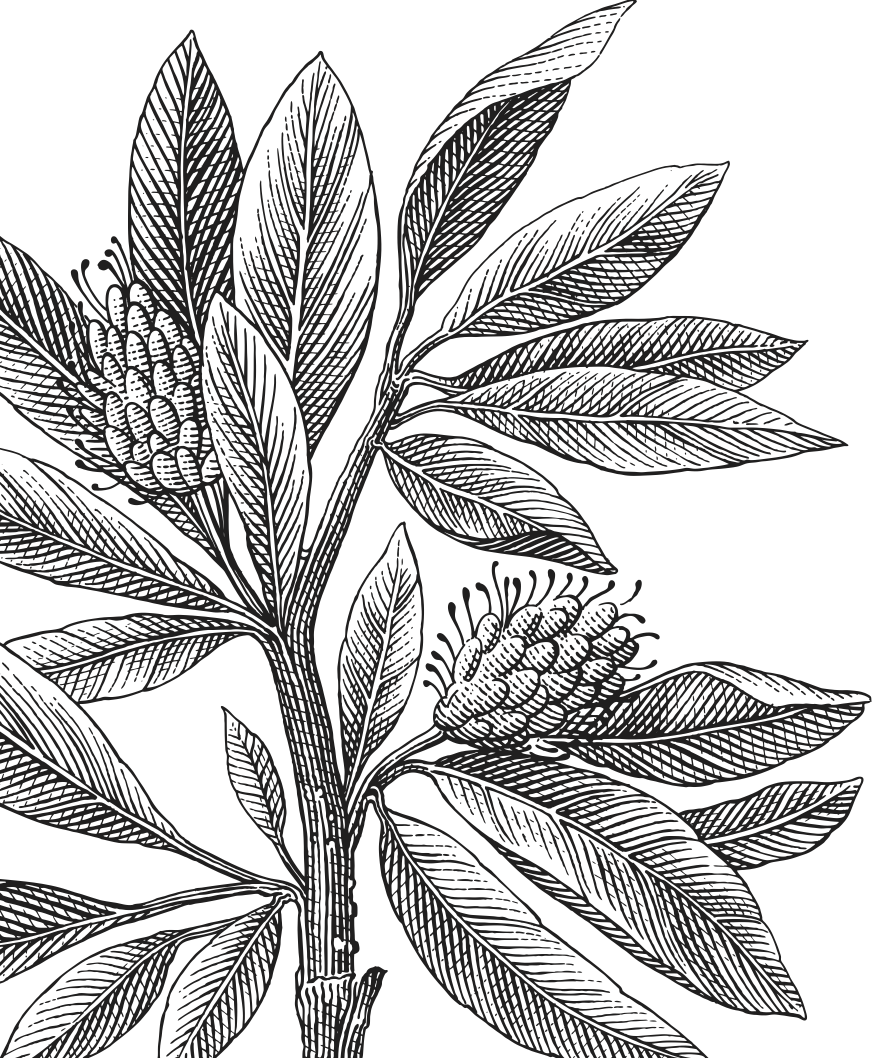
\includegraphics[keepaspectratio,scale=0.3]{img/lnu_etch.png} % Bakgrundsbild
    }
}
\newcommand\BackgroundPicLogo{
    \put(30,740){
    
\includegraphics[keepaspectratio,scale=0.10]{img/logo.png} % Logga i övre vänstra hörnet
    }
}

% In the following you can change the title of your document
\title{	
\vspace{-8cm}
\begin{sidebar}
    \vspace{10cm}
    \normalfont \normalsize
    \Huge Assignment 2\\ % Dokumentets typ, t.ex. Examensarbete
    \vspace{-1.3cm}
\end{sidebar}
\vspace{3cm}
\begin{flushleft}
    \LARGE Computer Networks - an introduction\\ % Dokumentets rubrik
 %   \it \LARGE Examensarbete under arbete % Dokumentets underrubrik
\end{flushleft}
\null
\vfill
\begin{textblock}{6}(9,11)
\begin{flushright}
\begin{minipage}{\textwidth}
\begin{flushleft} \large
\emph{Author:} John Herrlin\\ % Författare
\emph{Email: } jh222jx@student.lnu.se\\
\emph{Author:} Rasmus Sjostrom\\ % Författare
\emph{Email: } rs222kp@student.lnu.se\\
%\emph{Handledare:} Dr.~Foo \textsc{Bar}\\ % Handledare
%\emph{Examinator:} Dr.~Mark \textsc{Brown}\\ % Examinator
\emph{Semester:} VT2016\\ % Termin
\emph{Area:} Computer Science\\ % Ämne
%\emph{Level:} G2F\\ % Nivå
\emph{Coursecode:} 1DV701 % Kurskod
\end{flushleft}
\end{minipage}
\end{flushright}
\end{textblock}
}


\date{} % Dagens datum, tomt i detta fallet. Använd \today för dagens datum.

\begin{document}
\pagenumbering{gobble}
\newgeometry{left=5cm}
\AddToShipoutPicture*{\BackgroundPic} % Lägger in backgrundsbild på första sidan
\AddToShipoutPicture*{\BackgroundPicLogo} % Lägger in LNU-logga på första sidan
\maketitle % Skriv ut titeln
\restoregeometry
\clearpage
%------------------------------------------------------------------------------
%	Svensk och engelsk version av abstract
%------------------------------------------------------------------------------
{

%------------------------------------------------------------------------------
\newpage
\pagenumbering{gobble} % Stäng av sidnumrering för innehållsförteckningssidan
\tableofcontents % Innehållsförteckning
\newpage % Ny sida
\pagenumbering{arabic} % Påbörja sidnumrering på 1

%------------------------------------------------------------------------------
% This is where you write the report:
\section{Introduction}


The idea of our project was to build a small web framework, since we already
had to write the web server from scratch for the assignment. We figured this
to be a great opportunity to develop something we could continue working on
and learn more about since we consider it a very interesting field.\\
\\
Our goals with this small framework is to keep things as simple and modular
as possible, making it easy to expand or modify for further development.\\
\\
We are very well aware of the fact that the database parts were not a part
of the assignment, but to us it simply made sense to include this in the
project. Therefore, we have built a small ORM with a SQLite database found
in the db and domain modules. The reason for this was to be able to test and
use our PUT and POST methods naturally, as if we were performing them on a 
real life web server.\\
\\
We have saved the tcpclient in the code from the previous assignment.
The reson for this is that we used it for fuzzy testing against the endpoints.\\


\subsection{Workflow}

The small enumeration figure below describes the workflow of the webserver,
starting with a request and ending with a response being sent back.

\begin{enumerate}
  \item Parse an incoming request and create a Request object
  \item Send the request object to the URL handler, which will match the Request.uri with specified patterns
  \item If the requested uri matches a pattern, the URL handler will call the corresponding View, forward the request as an argument
  \item Depending on the called view, proper business logic will be executed. Thereon a response and body will be sent back to the client
\end{enumerate}

By following this model, adding new URLs and a corresponding View for that URL is extremely easy.\\

\section{Problem 1}

\begin{figure}[H]
    \centering  
    
\includegraphics[scale=0.5]{img/screenshots/htmlindex.png}
	\label{fig:htmlindex}
	\caption{Index page with imgs and CSS.}
\end{figure}


\begin{figure}[H]
    \centering  
    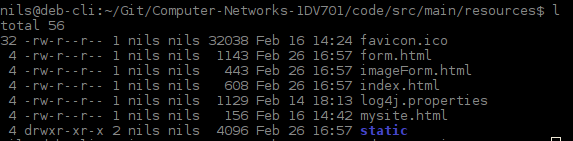
\includegraphics[scale=0.5]{img/screenshots/filesresourcefolder.png}
	\label{fig:filesresourcefolder}
	\caption{Resource folder, site root.}
\end{figure}


\begin{figure}[H]
    \centering  
    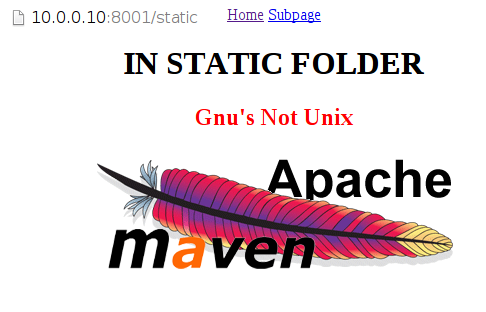
\includegraphics[scale=0.6]{img/screenshots/htmlstatic.png}
	\label{fig:htmlstatic}
	\caption{HTML document in static folder.}
\end{figure}


\section{Problem 2}

The table in ~\ref{fig:responsecodesandusage} describes different types of response codes that the server sends back to the client.
We table describes response codes that are both in the G task in Problem 1 and VG-task 1 in Problem 2.
The reason to have everything in one table and not to split them up if for the simplicity and readability.
Almost all of the response codes have figures and links to them are in the table.

\subsection{403}

We get this behavior when we try to post or put a form without being logged in.
Login is done via the endpoint: /login.

\begin{figure}[H]
    \centering  
    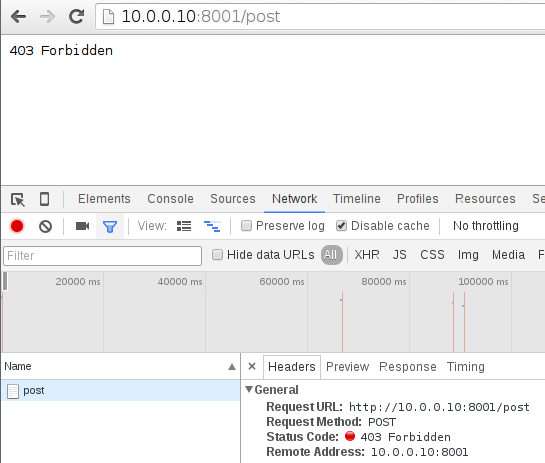
\includegraphics[scale=0.6]{img/screenshots/postnotallowed.png}
	\label{fig:postnotallowed}
	\caption{POST not allowed.}
\end{figure}

\subsection{404}

We get this behavior when we trying to access a endpoint that doesnt have any content.

\begin{figure}[H]
    \centering  
    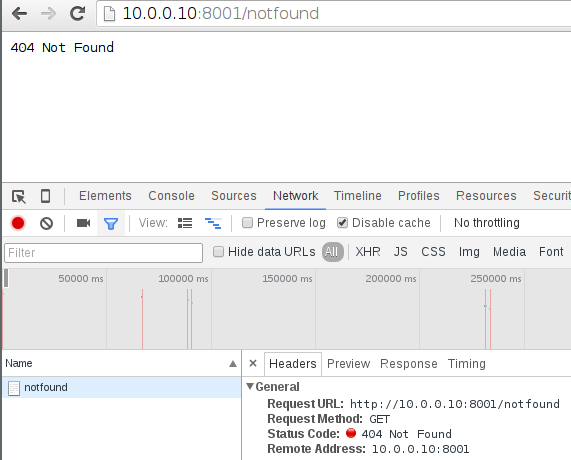
\includegraphics[scale=0.6]{img/screenshots/notfound.png}
	\label{fig:notfound}
	\caption{404 Not Found.}
\end{figure}

\subsection{500}

This behavior it hard to get from a web broser as is sends correct requests.
It appers if the server cant parse the request in a correct way it returns 500 Server Error.
A screenshot of a telnet caption can be found here, Figure~\ref{fig:response500servererror}


\subsection{VG-Task 1}

All responsecodes thats implemented can be found in Figure~\ref{fig:responsecodesandusage}


\subsection{VG-Task 2}

Both POST and PUT sends data to the server but are used in two different way.
PUT is used to update a resource on a specific endpoint.
In our server implementation we send data to /put/\{blog-uuid\}. The blog-uuid is the specific endoint where the resource should be updated.
POST is also connected to a endpoint, but doesnt need to have a specific location.
For example login, send data to the /login endpoint. The endpoint takes care of the data in the request, but we dont need to specify a specific id.
In out implementation we send data to /post to create a new blog  post.
The important part is that PUT should have a unique id for the resource and not POST.\\

\subsubsection{List all blog posts}

This endpoint lists all of the blog posts that we have in the db.

\begin{figure}[H]
    \centering  
    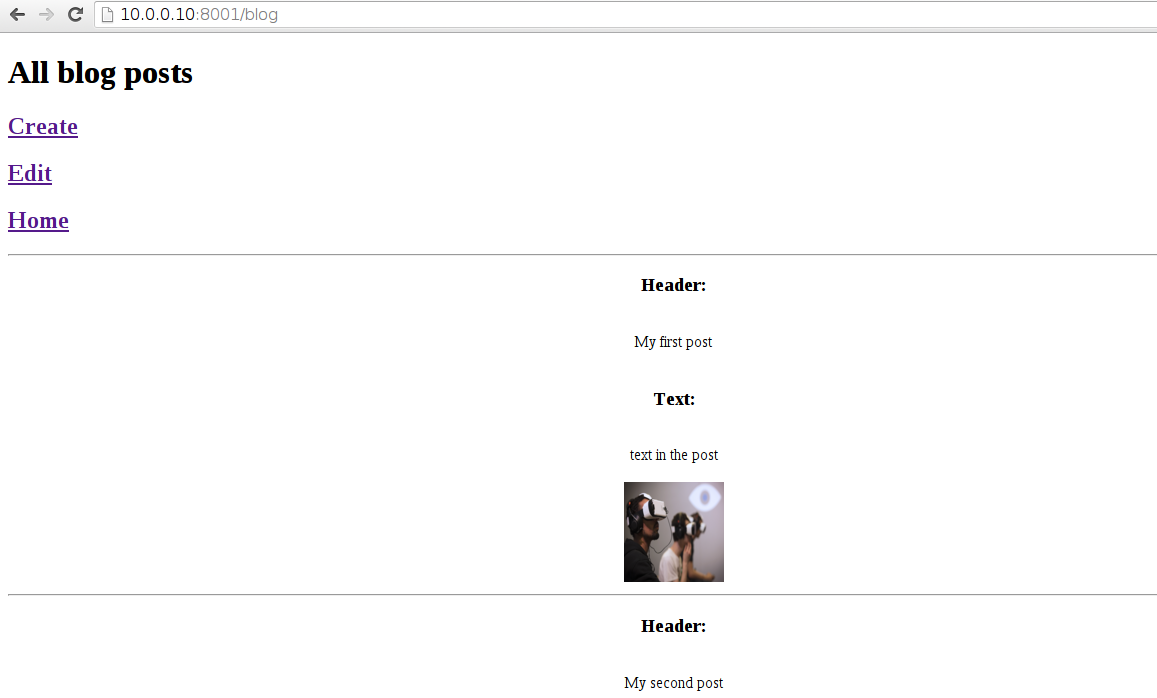
\includegraphics[scale=0.3]{img/screenshots/allblogposts.png}
	\label{fig:allblogposts}
	\caption{Method: GET, Endpoint: /blog, Comment: All blog posts in db.}
\end{figure}


\subsubsection{Create blog posts}

This endpoints provides a form for creating a new blog post.
When submiting the form the data is send to the /post endpoint and the form data in the request
body. The request method is POST.
The server parses the data and stores it in the db.
If the submit is correct the server sends back a document that redirect us to the /blog endpoint.

\begin{figure}[H]
    \centering  
    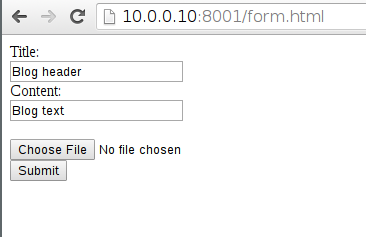
\includegraphics[scale=0.6]{img/screenshots/createblogpost.png}
	\label{fig:updateblogpost}
	\caption{Method: GET, Endpoint: /form.html, Comment: Create blog post.}
\end{figure}


\subsubsection{Update blog posts}

From this endpoint we can edit all of the blog posts.
The update is made with a PUT request to the endpoint /put/{blog-uuid}.
The server checks if we have a field in the form called \_method with the value put.
If the server finds that is sets the request as a PUT.
The server then tries to parse the data and update the blog entry by its uuid.
Response is a html document that redirects the user to the /blog endpoint.

\begin{figure}[H]
    \centering  
    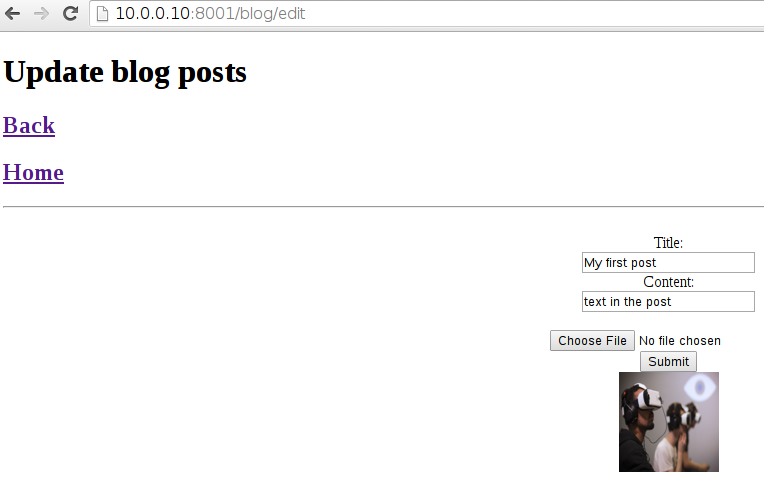
\includegraphics[scale=0.4]{img/screenshots/updateblogpost.png}
	\label{fig:updateblogpost}
	\caption{Method: GET, Endpoint: /blog/edit, Comment: Update blog posts.}
\end{figure}


\section{Problem 3}

Requesting a image from a URI within telnet gives back the compiled code of the image.

\begin{figure}[H]
  \centering
  \begin{tabular}{ | l | l | }
    \hline			
    Code & Usage \\
    \hline			
    200 & Many places where server handles response in a correct way. \\
    \hline			
    201 & When success with POST on /post Figure~\ref{fig:response201created} \\
    \hline			
    202 & When /login success Figure~\ref{fig:response202login} \\
    \hline			
    205 & When /logout success. Figure~\ref{fig:response205logout} \\
    \hline			
    400 & When not PUT on /put . Figure~\ref{fig:response400put} \\
    \hline			
    403 & When trying /post or /put before logged in (/login) before Figure~\ref{fig:response403forbidden} \\
    \hline			
    404 & When static file not found OR if url doesn match any Figure~\ref{fig:response404notfound} \\
    \hline			
    405 & When not POST on /post Figure~\ref{fig:response405methodnotallowed} \\
    \hline			
    500 & If we cant parse the request Figure~\ref{fig:response500servererror} \\
    \hline  
  \end{tabular}
  \label{fig:responsecodesandusage}
  \caption{Response codes and their usage.}
\end{figure}

\section{Screenshots}


\begin{figure}[H]
    \centering  
    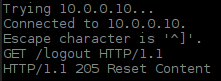
\includegraphics[scale=1]{img/screenshots/response205logout.png}
	\label{fig:response205logout}
	\caption{Method: GET, Endpoint: /logout, Response: 205 Reset Content}
\end{figure}


\begin{figure}[H]
    \centering  
    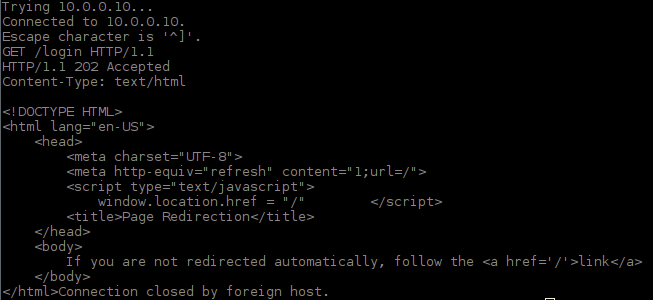
\includegraphics[scale=0.6]{img/screenshots/response202login.png}
	\label{fig:response202login}
	\caption{Method: GET, Endpoint: /login, Response: 202 Accepted}
\end{figure}


\begin{figure}[H]
    \centering  
    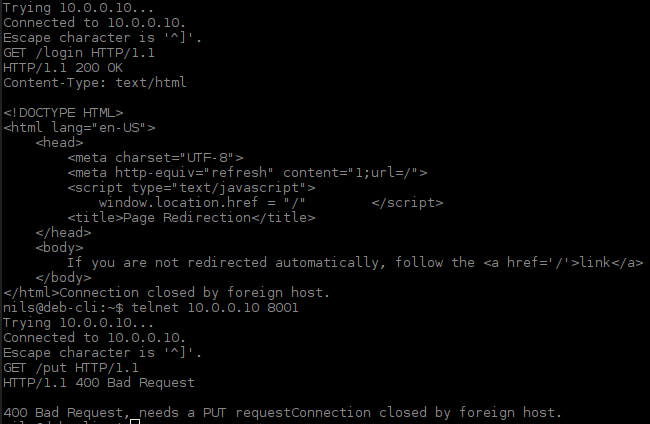
\includegraphics[scale=1]{img/screenshots/response400put.png}
	\label{fig:response400put}
	\caption{Method: GET, Endpoint: /put, Response: 400 Bad Request}
\end{figure}


\begin{figure}[H]
    \centering  
    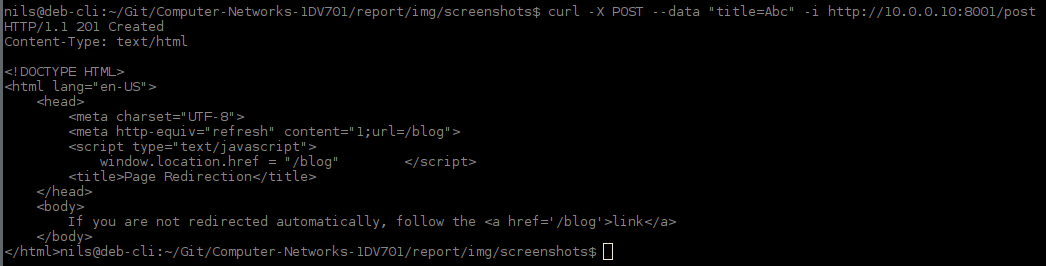
\includegraphics[scale=0.40]{img/screenshots/response201created.png}
	\label{fig:response201created}
	\caption{Method: POST, Endpoint: /post, Response: 201 Created}
\end{figure}


\begin{figure}[H]
    \centering  
    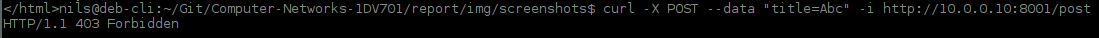
\includegraphics[scale=0.40]{img/screenshots/response403forbidden.png}
	\label{fig:response403forbidden}
	\caption{Method: POST, Endpoint: /post, Response: 403 Forbidden}
\end{figure}


\begin{figure}[H]
    \centering  
    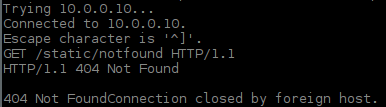
\includegraphics[scale=0.70]{img/screenshots/response404notfound.png}
	\label{fig:response404notfound}
	\caption{Method: GET, Endpoint: /static/notfound, Response: 404 Not Found}
\end{figure}


\begin{figure}[H]
    \centering  
    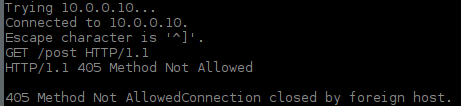
\includegraphics[scale=0.70]{img/screenshots/response405methodnotallowed.png}
	\label{fig:response405methodnotallowed}
	\caption{Method: GET, Endpoint: /post, Response: 405 Method Not Allowed}
\end{figure}


\begin{figure}[H]
    \centering  
    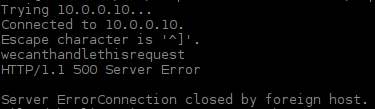
\includegraphics[scale=0.80]{img/screenshots/response500servererror.png}
	\label{fig:response500servererror}
	\caption{Method: ?, Endpoint: ?, Response: 500 Server Error}
\end{figure}


\section{How To Run/Build}

Import the project as a maven project in an IDE.
Download maven dependencies.
Run se.jherrlin.run.Main with arguments: -m tcpserver\\


%------------------------------------------------------------------------------
%\bibliographystyle{IEEEtran}
% Here you will have to put your bibliography
%% \newpage
%% \bibliography{ieeedb.bib}{}
%% \bibliographystyle{IEEEtran}


\end{document}
